\section{LED et résistance (4 points)}

Lorenzo réalise le circuit suivant en utilisant une résistance de 50 $\Omega$ . \'A l'aide d'un voltmètre il mesure la tension aux bornes du générateur ($U_G$)et de la LED ($U_{DEL}$) .

\begin{center}
	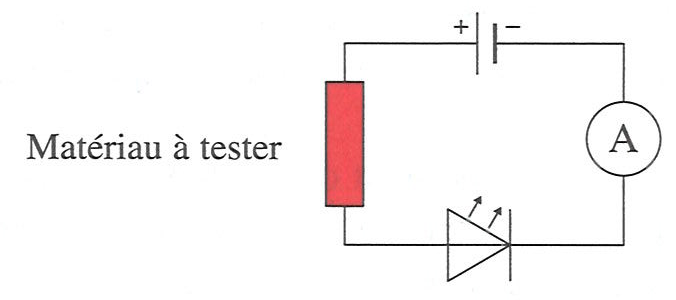
\includegraphics[scale=0.2]{img/circuit}
\end{center}

\begin{questions}
	\question[1] Comment sont branchés la LED et la résistance ?
	
	\question[1] Calculer la tension aux bornes de la résistance ($U_R$) ?
	
	\question[1] Calculer l'intensité du courant qui traverse la résistance ($I_R$) ?
	
	\question[1] En déduire l'intensité du courant qui traverse la LED.
\end{questions}